% RESULTADOS-------------------------------------------------------------------
%Cada capítulo deve conter uma pequena introdução (tipicamente, um ou dois parágrafos) que deve deixar claro o objetivo e o que será discutido no capítulo, bem como a organização do capítulo.
%\chapter{ANÁLISE E DISCUSSÃO DOS RESULTADOS}
\chapter{RESULTADOS}
\label{Chap:Resultados}

Este capítulo apresenta o que foi obtido como resultado deste trabalho, e as experiências do autor durante o desenvolvimento do sistema de atualização de \firmware\ over-the-air. Primeiro será apresentado os resultados mostrando como é um processo de atualização realizado com sucesso e em seguida discutido o uso, vantagens e desvantagens do sistema. 

\section{PROCESSO DE ATUALIZAÇÃO DE FIRMWARE}
Aqui é presentado todo o processo de atualização feito para comprovar o funcionamento do sistema desenvolvido neste trabalho, com isso é abordado desde a inicialização do \firmware\ 1 com sua mensagem de apresentação, a disponibilização do \firmware\ 2 no servidor, o processo de atualização, a inicialização do \firmware\ 2 na plataforma embarcada STM32F746G e sua mensagem de apresentação.

\subsection{ESTADO INICIAL DO MICROCONTROLADOR}
Inicialmente é gravado no microcontrolador o \bootloader\ e depois o \firmware\ 1, com isso temos a memória flash preenchida separadamente, visto que definimos áreas diferentes para aplicação e \bootloader\ no arquivo de linker, assim temos o estado inicial da memória do microcontrolador no inicio do teste.

Com o \bootloader\ e \firmware\ 1 gravados no \textit{hardware}, já é possível fazer a primeira inicialização do sistema, com a reinicialização do \textit{hardware} o sistema inicializa o \bootloader\ para poder dar sequência de atualização ou salto para a aplicação. A \autoref{memoriaflash} mostra a configuração de memória flash do microcontrolador.

\begin{figure}[H]
    \scriptsize
     \centering
     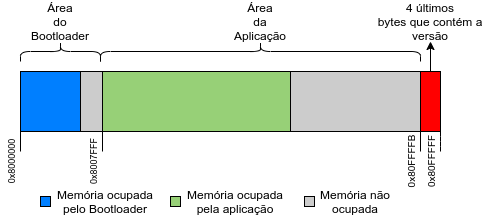
\includegraphics[scale=0.9]{dados/figuras/flash_ocupation.png}
     \caption{Imagem ilustrativa da configuração da memória flash. \newline Fonte: Autoria própria.}
     \label{memoriaflash}
\end{figure}

\subsection{INICIALIZAÇÃO DO BOOTLOADER}
Após todos os processos de inicialização o \bootloader\ é executado. Como o intuito é que o \bootloader\ não ocupe muito espaço da memória flash do microcontrolador, e de forma que se adapte para todos os tipos de microcontroladores da familia STM32, não foi previsto nenhum tipo de sinalização durante sua operação. Dessa forma, a substituição do \firmware\ e o salto para a aplicação são executadas sem nenhuma informação visual para o usuário.

Durante sua execução o \bootloader\ verifica a versão do \firmware\ atual e o compara com a versão que está no cartão SD, caso a versão atual for menor ou não seja encontrada a nova versão do \firmware\, o \bootloader\ inicializa o \firmware\ que está na memória flash. Como neste caso de teste o cartão SD se encontra vazio, o \bootloader\ assume que não há nenhuma atualização a ser efetuada, assim ele inicializa a sequência de salto para a aplicação. 

\subsection{INICIALIZAÇÃO DO FIRMWARE 1}
Com a inicialização da aplicação efetuada pelo \bootloader, são executadas todas as inicializações de drivers, das bibliotecas utilizadas pelo \firmware\ 1, e assim inicializado o sistema operacional FreeRTOS, e exibida via UART a mensagem de confirmação de montagem do driver do cartão SD e a mensagem de apresentação contendo a versão do \textit{software} atual e o sua frase de identificação. A partir da impressão dessas frases o sistema operacional iniciará a tarefa OTA.

\subsection{OTA}
Ao iniciar a função OTA será buscado no servidor o arquivo contendo a versão do \firmware\ 2, com esse arquivo baixado ele fará a comparação com a versão atual do \firmware\ e caso necessário irá fazer o \download\ do novo \firmware, e do arquivo contendo o hash deste \firmware. Tendo esses arquivos salvos no cartão SD ele irá fazer o hash do \firmware\ baixado e verificar assim a integridade do arquivo baixado. Caso todos os processos ocorram com sucesso ele irá fazer com que esses arquivos permaneçam no cartão SD e iniciará o processo de salto para o \bootloader, que encerra todos os driver e o sistema operacional e pula para a região do \bootloader\ para o executar. Todo esse processo pode ser visto na \autoref{Firmware1OTA}.

\begin{figure}[H]
    \scriptsize
     \centering
     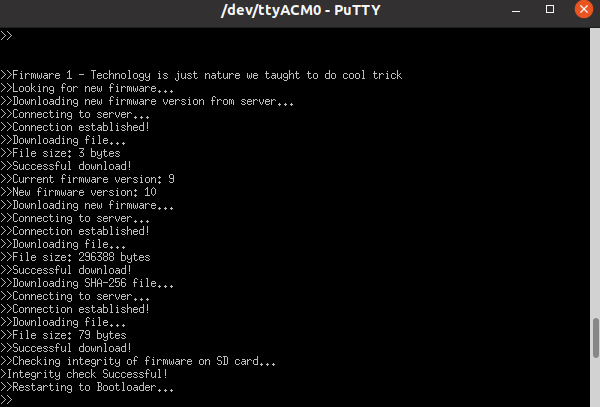
\includegraphics[scale=0.9]{dados/figuras/Firmware1.png}
     \caption{Processo de atualização realizado pela função OTA no \textit{firmware} 1 \newline Fonte: Autoria própria.}
     \label{Firmware1OTA}
\end{figure}

\subsection{REINICIALIZAÇÃO DO SISTEMA PARA O BOOTLOADER}
O \bootloader\ é inicializado novamente, mas agora ele consegue achar um arquivo de versão escrito no cartão SD, com isso fazer a comparação com a versão de \firmware\ e como a versão encontrada no cartão SD é maior que a escrita na flash, ele iniciará o processo de troca de \firmware.
Após a troca de \firmware\ ele escreverá nas 4 últimas posição da memória a versão do novo \firmware, fazendo com que atualização seja concluída com sucesso, assim podendo novamente fazer o processo de pulo para a aplicação.

\subsection{INICIALIZAÇÃO DO FIRMWARE 2}
Após o pulo para aplicação efetuada pelo \bootloader\ após a atualização são executadas todas as inicializações de drivers, das bibliotecas utilizadas pelo \firmware\ 2, e assim inicializado o sistema operacional, exibida a mensagem de confirmação de montagem do driver do cartão SD e a mensagem de apresentação contendo a versão do \textit{software} atual e a sua nova frase de identificação como pode ser observado na \autoref{fraseidentificacao2}. Assim concluindo com sucesso um processo de atualização de \firmware.

\begin{figure}[H]
    \scriptsize
     \centering
     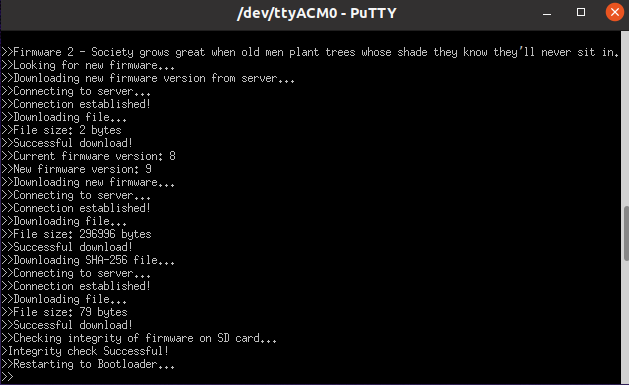
\includegraphics[scale=0.9]{dados/figuras/Firmware2.png}
     \caption{\textit{Firmware} 2 iniciado com processo de atualização. \newline Fonte: Autoria própria.}
     \label{fraseidentificacao2}
\end{figure}

\section{TRATAMENTOS DE ERROS IMPLEMENTADOS}
Durante o processo de atualização e obtenção de arquivos diversos erros podem ocorrer, desde quedas de energia, a falhas de conexão com o servidor. Para evitar que esses erros deixem a plataforma embarcada em um estado não conhecido foram implementados diversos tratamentos de erros que serão explanados nessa sessão.
\subsection{FALHA AO ENCONTRAR ARQUIVOS NO SERVIDOR}
Caso o cliente OTA não conseguir encontrar no servidor um dos arquivos que são necessários para a atualização, como o arquivo contendo o número versão, ou o arquivo contendo a nova versão do \firmware, ou mesmo o arquivo com o hash desse \firmware. O cliente OTA tem a capacidade de detectar esse tipo de erro e apresentar ao usuário este erro, tornando fácil a identificação dessa falha. A \autoref{erro_404} apresenta como o cliente OTA informa o usuário do erro que ocorreu.
\begin{figure}[H]
    \scriptsize
     \centering
     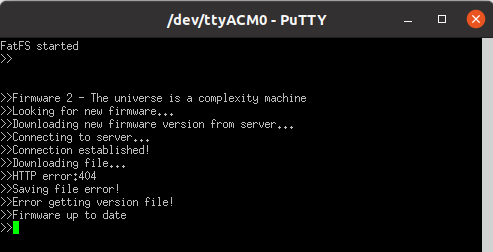
\includegraphics[scale=1.2]{dados/figuras/404.png}
     \caption{Erro ao não encontrar arquivo no servidor. \newline Fonte: Autoria própria.}
     \label{erro_404}
\end{figure}

\subsection{FALHA AO COMPARAR HASH}
Após o \download\ da última versão do \firmware, o cliente OTA gera um hash utilizando a função de hash sha-256 que a biblioteca MbedTLS fornece, esse hash é comparado com o que foi obtido do servidor para garantirmos que o \firmware\ obtido está integro e não corrompido. Caso essa comparação falhe, uma mensagem é mostrada para o usuário, essa mensagem pode ser observada na \autoref{erro_hash}.
\begin{figure}[H]
    \scriptsize
     \centering
     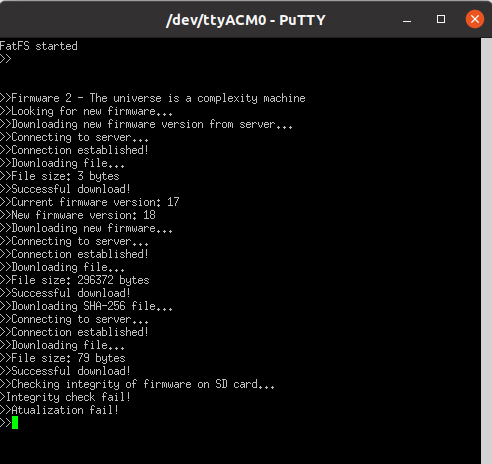
\includegraphics[scale=1.2]{dados/figuras/hash_error.png}
     \caption{Erro ao comparar hash do servidor com a hash gerada a partir do \firmware\ obtido do servidor. \newline Fonte: Autoria própria.}
     \label{erro_hash}
\end{figure}
\subsection{QUEDA DE ENERGIA DURANTE PROCESSO DE ATUALIZAÇÃO}
Caso exista uma queda de energia, ou algo que faça com que o microcontrolador seja reiniciado durante o processo de escrita do \firmware\ na flash, que ocorre no \bootloader, o sistema tem a capacidade de identificar este erro a partir do número de versão que está presente no fim da memória. No evento desse valor ser igual a 0xFFFFFFFF, significa que a última operação de escrita da flash não foi concluída com sucesso, assim é necessário que ela seja refeita. Assim o \bootloader\ executa uma rotina de reinicialização do sistema caso não encontre o \firmware\ para realizar a atualização no cartão SD, e caso encontre ele executa a atualização e salta para a nova aplicação.


\section{DISCUSSÃO}
Os resultado obtidos mostraram que o sistema de atualização de \textit{firmware Over-The-Air} proposto neste trabalho funciona, e que todo o processo desde a verificação de uma aplicação válida feita pelo \bootloader, seu processo de atualização e as obtenções e verificações de arquivos da API de atualização OTA ocorrem com sucesso.

Como o \bootloader\ ocupa 22 kbytes de espaço na memória flash, pode ser utilizado por diversas placas da familia de microcontroladores STM32 que possuam um setor da memória maior que esse espaço.
No entanto, o \bootloader\ proposto tem como único objetivo, substituir o \firmware\ na memória flash do microcontrolador por um versão atualizada, desde que esse novo \firmware\ esteja no cartão SD. Já o código que realiza o procedimento de verificação e \download\ desse novo \firmware\ a partir de um servidor na internet para o cartão SD é conhecido por atualização \textit{over-the-air}. 

A atualização OTA é executada por uma tarefa instalada no sistema e utiliza várias bibliotecas para sua operação. O conjunto de aplicação e bibliotecas da atualização OTA proposta ocupou 294kB de memória de programa em um microcontrolador ARM Cortex-M7, utilizando o compilador gcc. É importante destacar que as bibliotecas que adicionam suporte a concorrência, sistema de arquivos, comunicação TCP/IP e segurança por TLS podem e devem ser utilizadas pelo código de aplicação, sendo consideradas bibliotecas compartilhadas.
Considerando que o microcontrolador utilizado possui 1024kB de memória FLASH, a aplicação do usuário ainda teria 698 kbytes restante na memória de programa, se já subtrairmos os 32 kbytes reservados para o \bootloader. 


As bibliotecas utilizadas ocupam a maior parte destes 294kB, como pode ser verificado no arquivo de mapeamento de memória gerado na compilação do projeto. Nesse arquivo pode-se identificar a quantidade de memória de dados e de programa utilizada por cada uma das bibliotecas incluídas na projeto. Considerando a memória de programa, a biblioteca FatFS ocupa cerca de 8 kbytes de memória, a LwIP em torno de 48 kbytes de memória flash e por fim a MbedTLS que ocupa aproximadamente 130 kbytes de memória, sendo essa a biblioteca que mais ocupa espaço na memória flash. Temos então que aproximadamente 186 kbytes do \firmware\ é ocupados pelas bibliotecas, assim dois terços do \firmware\ desenvolvido é ocupado por funções e outras definições das bibliotecas. A API de atualização desenvolvida ocupa por volta de 2 kbytes, ficando o restando do \firmware\ ocupado pelo sistema operacional, outras funções do HAL e demais códigos de inicialização.

A ocupação de memória de programa poderia ser reduzida drasticamente caso não fosse utilizada a criptografia e autenticação provida pela biblioteca MbedTLS, devido a sua ocupação de 135 kB de memória flash. No entanto, a segurança na atualização de um \firmware\ é extremamente importante para se garantir a origem e integridade do novo \firmware. Outra possibilidade que não foi abordada neste trabalho é a otimização da compilação com o objetivo de se diminuir a ocupação da memória flash, que poderia diminuir o tamanho total do código de 294 kbytes para cerca de 260 kbytes. Outra otimização que pode ser feita é a otimização com o intuito de se aumentar o desempenho, fazendo com que o código ocupe aproximadamente de 350 kbytes.

Outra análise importante de ser feita é o uso de memória RAM dessas aplicações, em que podemos observar que essas bibliotecas acabam por tomar muita memória RAM do sistema, assim como acontece na memória flash. A quantidade de memória RAM gasta pela FatFS fica em torno de 20 bytes tornando ela a biblioteca que menos ocupa espaço em ambas as memórias. É seguida pela MbedTLS que consome cerca de 9 kbytes, e então pela LwIP que por ter que criar uma pilha de protocolos chega a ocupar aproximadamente 40 kbytes de memória RAM. Além disso temos o \textit{heap} do FreeRTOS que é utilizado para pilhas de tarefas, alocação dinâmica de memória, semáforos, filas, etc. Durante o processo de atualização, dos 186 kbytes disponíveis na \textit{heap}, 65 kbytes são alocados dinamicamente para as funções das bibliotecas.

Dessa maneira observamos que o sistema fica ainda menos portável para \textit{hardwares} menos robustos, visto que o consumo de memória RAM das bibliotecas é muito alto, onde somente observando as bibliotecas chega a 50 kbytes. Outra observação importante é que nos \textit{firmwares} desenvolvidos foi utilizado o sistema operacional FreeRTOS que ocupa 4 kB de memória RAM, e tem 186 kB de \textit{heap}. Porém esse número pode ser reduzido se diminuirmos o \textit{heap} do sistema operacional. Enquanto outras funções e inicializações ocupam mais 29 kbytes da memória RAM. Com isso obtemos que cerca de 269 kbytes dos 340 kbytes de memória RAM global disponíveis no microcontrolador STM32F746G são ocupados pelo \textit{firmware}.

Com essa informação sobre o tamanho dos arquivos, é possível notar que este sistema de atualização não é tão portável quanto se esperava no inicio deste trabalho, visto que só para ter um sistema de atualização funcional precisamos que o \textit{hardware} em que se deseja ter esse sistema tenha ao menos 512 kbytes de memória flash, e no mínimo 115 kbytes de memória RAM, assim diminuindo muito a quantidade de microcontroladores que poderiam utilizar este sistema. Esse sistema acaba sendo muito proveitoso para aplicações que já utilizam essas bibliotecas, pois assim não precisariam incluir novamente as bibliotecas FATFS, MbedTLS, LWIP, como é o caso de dispositivos de IoT. De forma geral é possível observar os gastos de memórias com as bibliotecas na \autoref{memorias}. \newline


\begin{table}[H]
    \scriptsize
    \centering
    \begin{tabular}{|c|c|c|}
    \hline
    \textbf{Biblioteca} & \textbf{Memória RAM} & \textbf{Memória flash} \\ \hline
    \textbf{FatFs}      & 20 bytes             & 8 kbytes               \\ \hline
    \textbf{LwIP}       & 40 kbytes            & 48 kbytes              \\ \hline
    \textbf{MbedTLS}    & 9 Kbytes             & 130 kbytes             \\ \hline
    \end{tabular}
    \caption{Ocupação das memórias do microcontrolador STM32F746NGH6 pelas bibliotecas. \newline Fonte: Autoria própria.}
    \label{memorias}
    \end{table}

Ainda assim é possível afirmar que o sistema cumpre com o objetivo geral e específicos propostos, visto que o sistema é capaz de efetuar a atualização da plataforma embarcada STM32F746NGH6 da forma proposta e ainda é capaz de identificar quando houve falhas em seu sistema de atualização e se recuperar de forma autónoma dessas falhas. Os códigos do \bootloader\ e do sistema de atualização OTA desenvolvidos nesse trabalho podem ser encontrados no seguinte link do \href{https://github.com/GustavoCorrea-GC/OTA}{GitHub}.   
